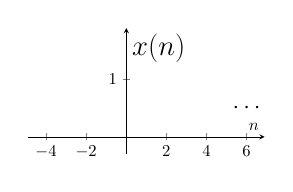
\begin{tikzpicture}[scale=0.6,transform shape]
    \begin{axis}[
        x=0.035\textwidth,y=0.1\textwidth,
    	axis y line=center,
    	axis x line=middle,
    	xlabel=$n$,ylabel={\LARGE $x(n)$},
    	xmin=-4.9,xmax=6.9,
    	ymin=-0.3,ymax=1.9,
    	xticklabel style = {xshift=0},
    	ytick = {0, 1},
        yticklabel style = {yshift=.1},
    	]
    	\discretedelta{-4}{0.1};
    	\discretedelta{-3}{0.1};
        \discretedelta{-2}{1};
        \discretedelta{-1}{1};
        \discretedelta{0}{1};
        \discretedelta{1}{1};
        \discretedelta{2}{1};
        \discretedelta{3}{1};
        \discretedelta{4}{1};
        \discretedelta{5}{1};
    	\node at (6,0.5) {\Large $\cdots$};
    \end{axis}
\end{tikzpicture}